
\title{Rover}

\date{\today}

\author{Alex Wallar}

\documentclass[12pt]{article}

\usepackage{amsmath}

\usepackage[pdftex]{graphicx}

\usepackage{relsize}

\usepackage{float}

\usepackage{algorithm}

\usepackage[noend]{algorithmic}

\floatstyle{ruled} \newfloat{program}{thp}{lop} \floatname{program}{Structure}

\newcommand{\Normal}[3]{\mathcal{N}(#1, #2, #3)}

\newcommand{\Acronym}[1]{\ensuremath{{\small{\texttt{#1}}}}}
\newcommand{\Constant}[1]{\ensuremath{\small{\texttt{#1}}}}
\newcommand{\Rover}{\Acronym{Rover}}
\newcommand{\Keeper}{\Acronym{Keeper}}
\newcommand{\False}{\Constant{false}}
\newcommand{\True}{\Constant{true}}
\newcommand{\Symbol}[1]{\ensuremath{\mathcal{#1}}}
\newcommand{\Function}[1]{\ensuremath{{\small \textsc{#1}}}}
\newcommand{\Var}[1]{\ensuremath{{\small{\textsl{#1}}}}}
\newcommand{\argmax}[1]{\underset{#1}{\operatorname{arg}\,\operatorname{max}}\;}
\newcommand{\Max}[1]{\underset{#1}{\operatorname{max}}\;}
\newcommand{\grad}[1]{\underset{#1}{\operatorname{\Function{GradientDecent}}}\;}
\newcommand{\s}{\textbf{s}}
\newcommand{\fig}[1]{\textbf{Figure \ref{fig:#1}}}

\usepackage{fancyvrb}

\begin{document}

\maketitle

\newpage

% \tableofcontents

% \newpage

\section{Introduction}

Unmanned aerial vehicles, such as quadrotors, are becoming a cheap and
feasible way to provide persistent monitoring of an area even when monitoring
that area comes with a risk of the quadrotor being detected by possibly
hostile parties. These quadrotors are left unattended and need to be able to
plan their movements autonomously such that they maximize the quality of their
sensors and maintain as much sensor coverage as possible, whilst minimizing the
risk of being apprehended. The autonomous planning also needs to take into
account that some quadrotors will be dispatched from the swarm to follow
certain targets of interest. The planning algorithm should be able to
organically readjust the swarm such that maximum sensor quality and minimum
risk are preserved.

The proposed solution, Rover, provides a method of organically readjusting the
swarm to fill the search space whilst maximizing sensor quality and sensor
coverage while minimizing the risk of detection by hostile targets by combining
dynamic potential fields and non-linear optimization techniques.

\section{Rover}

Rover is an planning algorithm that seeks to maximize the sensor quality and
sensor coverage for a group of quadrotors, whilst minimizing the risk of a
quadrotor being detected by a possibly hostile enemy. This is done by
splitting the planning into two different parts, planning for the 2-D plane to
promote sensor coverage and planning for the altitude by minimizing risk and
maximizing sensor quality.

\subsection{2-D Planning}

\begin{figure}[ht]

    \begin{center}

        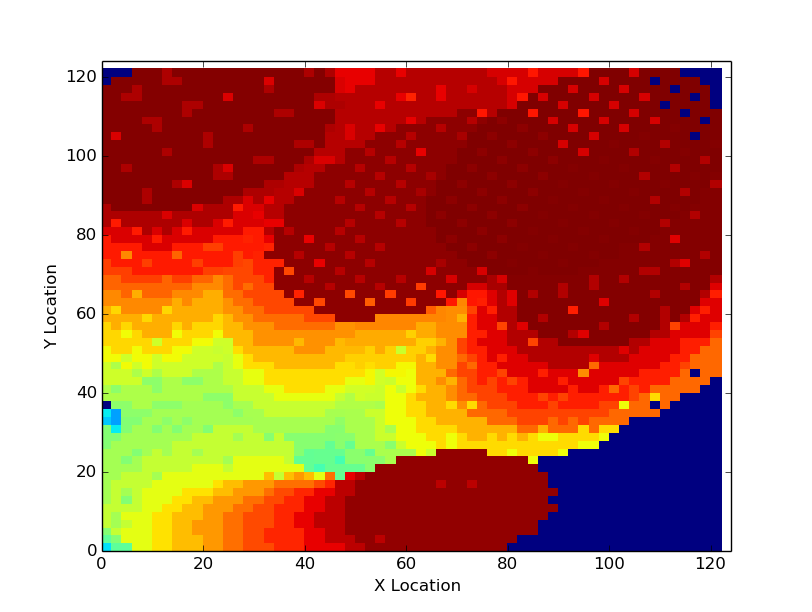
\includegraphics[width=\linewidth]{figs/timegrid_map.png}

    \end{center}

    \caption{An instance of the time grid where blue represents locations that
        have not been visited in a large amount of time and where red
    represents locations that have just been visited}
    
    \label{fig:timegrid}

\end{figure} 

For 2-dimensional planning, Rover needs to make sure that the group of
quadrotors fills the search space and guarantee that no one part of the space
goes too long without being surveyed. This is done by discretizing the space
into a grid (in this paper called a time grid and referred to as $\mathcal{T}$.
Whenever a box in the grid has been covered by a sensor on any quadrotor in the
group, the current time is stored in that box.  For the quadrotors to move in
the $xy$ plane, each quad will sample a given number of segments along the
sensing ellipse and move towards the segment whose average time is the least.
This simple rule has extreme emergent properties for the swarm.  Since the
swarm shares the same grid, the quads will act cooperatively to fill the space
without having to provide much guidance.  An instance of the time grid for a
given instance in time is shown in \fig{timegrid}.  Also, this planning is not
dependent on how many quads there are in the swarm.  If a quad leaves the
swarm, it would simply no longer update the time grid. The other quads would
have no knowledge that it left and would still be able to plan accordingly. 

\begin{algorithm}[ht]

\caption{$\Function{GetDirection}(q, \beta, \phi, \mathcal{T})$}

\label{algo:2dplanning}

\begin{algorithmic}[1]

\setcounter{ALC@line}{0}

\vspace*{1mm}


\STATE $t_{s} \leftarrow 0$
\STATE $\mathcal{P} \leftarrow \Function{Set()}$
\STATE $\zeta \leftarrow \Function{GetInnerSearchRange}()$
\STATE $S_{\theta} \leftarrow \Function{GetUniformSamples}(0, 2 \pi)$

\FOR{$\theta \in S_{\theta}$}

\STATE $S_{\omega} \leftarrow \Function{GetUniformSamples}(\theta - \zeta, \theta + \zeta)$

\FOR{$\omega \in S_{\omega}$}

\STATE $A_{M} \leftarrow q.\Var{z} \cdot (\tan{(\phi + q.\alpha)} - \tan{\phi}) + \epsilon$
\STATE $A_{m} \leftarrow q.\Var{z} \cdot \frac{\tan{q.\alpha}}{\cos{\phi}} + \epsilon$

\STATE $x \leftarrow q.\Var{z} \cdot \tan{(\phi - q.\alpha)} + A_{M} \cdot (1 + \cos{\omega})$
\STATE $y \leftarrow A_{m} \cdot \sin{\omega}$

\STATE $\begin{bmatrix}
    \hat{x} \\[0.2em]
    \hat{y}
\end{bmatrix} \leftarrow \begin{bmatrix}
    \cos{\beta} & -\sin{\beta} \\[0.2em]
    \sin{\beta} & \cos{\beta}
\end{bmatrix} \cdot \begin{bmatrix}
    x \\[0.2em]
    y
\end{bmatrix} + \begin{bmatrix}
    q.\Var{x} \\[0.2em]
    q.\Var{y}
\end{bmatrix}$

\STATE $t_{s} \leftarrow t_{s} + \mathcal{T}[\hat{x}, \hat{y}]$
\STATE $\mathcal{P}.\Var{add}(\hat{x}, \hat{y})$

\ENDFOR

\ENDFOR

\STATE $\bar{x} \leftarrow 0$
\STATE $\bar{y} \leftarrow 0$

\FOR{$(x, y) \in \mathcal{P}$}

\STATE $w \leftarrow \frac{\mathcal{T}[x, y]}{t_{s}}$
\STATE $\bar{x} \leftarrow \bar{x} + w \cdot x$
\STATE $\bar{y} \leftarrow \bar{y} + w \cdot y$

\ENDFOR

\RETURN $(\begin{bmatrix}
    \bar{x} - q.\Var{x} & \bar{y} - q.\Var{y}
\end{bmatrix} ^ T, \mathlarger{\frac{t_s}{|\mathcal{P}|}})$

\end{algorithmic}
\end{algorithm}



The quadrotors used in simulation have a variable camera angle. This means that
instead of simply having a down facing camera, the quadrotor can have the
camera at an angle, $\phi$. This means that the camera's projection onto the
$xy$ plane is not a circle but an ellipse. The major and minor axis of the
ellipse are, $ A_M(z, \phi) = z \cdot \tan{(\phi + \alpha)} - z \cdot
\tan{\phi} $ and $ A_m(z, \phi) = \frac{z \cdot \tan{\alpha}}{\cos{\phi}} $
where $z$ is the height of the quadrotor, $\phi$ is the camera angle and
$\alpha$ is the viewing angle.

Since an ellipse is not symmetrical for every angle, orientation cannot be
ignored.  This means that the 2-D planner must plan for not only $x$ and $y$
but also an orientation, $\beta$. Also, for completeness, we assume that the
camera angle, $\phi$, is also dynamic and can be set by the planner. In order
to plan the movements, we sample viable new orientations and camera angles,
each time determining the new $x$ and $y$ direction to go in.  Then once the
sampling has completed, we choose a $(x', y',
\beta', \phi')$ that would lead the quadrotor to a configuration that not has
been sensed in the largest amount of time. More formally, we would like to
minimize,

$$ E(\s) = \int_{\s_{\theta} - \zeta}^{\s_{\theta} + \zeta}
\mathcal{T}(e_x(\s, \omega), e_y(\s, \omega)) \cdot \sqrt{
    \Big(\frac{\partial e_x}{\partial \omega}\Big) ^ 2 +
\Big(\frac{\partial e_x}{\partial \omega}\Big) ^ 2} \;d\omega$$

where $E$ is the line integral on the curvature of the sensing ellipse within a
range centered at the currently sampled heading, $\theta$ in which the surface
being integrated upon is the time grid, $\mathcal{T}$. The variable $\zeta$
represents the interval of the integral and governs the size of the line
segment sampled when determining the new heading. The vector, $\s =
\langle z, \theta, \beta, \phi \rangle$ in $E$ holds the current state
of the altitude, heading, orientation, and camera angle respectively. The
equations,

$$
\begin{bmatrix}
    e_x(\s, \omega) \\[0.2em] e_y(\s, \omega)
\end{bmatrix} = \begin{bmatrix} \cos{\s_{\beta}} & -\sin{\s_{\beta}} \\[0.2em]
    \sin{\s_{\beta}}
& \cos{\s_{\beta}} \end{bmatrix}\cdot \begin{bmatrix} \s_z \cdot 
    \tan(\s_{\phi} - \alpha) +
    A_M(\s_z, \s_{\phi}) \cdot (1 + \cos{\omega}) + \epsilon \\[0.2em]
    A_m(z, \s_{\phi}) \cdot
\sin{\omega} + \epsilon \end{bmatrix} $$

%$$ E(z, \theta, \beta, \phi) = \mathlarger{\sum_{(x, y) \in S(z,
%            \theta, beta, \phi)}{\mathcal{T}[x, y]}}$$

%where $S$ is the set of points on the current line segment on the sensing
%ellipse that we are checking for a given $\theta$. More formally $S$ is defined
%as,
%
%$$ S(z, \theta, \beta, \phi) = \left\{ R(\beta) \cdot \begin{bmatrix} z \cdot
%       \tan(\phi - \alpha) + A_M(z, \phi)
%           \cdot (1 + \cos{\omega}) \\[0.2em]
%  A_m(z, \phi) \cdot \sin{\omega} \end{bmatrix} : \omega \in [\theta - \zeta, \theta + \zeta] \right\}$$

% where
%$$R(\beta) = \begin{bmatrix}
%\cos{\beta} & -\sin{\beta} \\[0.2em] \sin{\beta} & \cos{\beta} \end{bmatrix}$$

are parametric equations representing points on the sensing ellipse given a
quadrotor state, $\s$, along with an angle parameter, $\omega \in [0, 2\pi]$.

Therefore to determine the direction, $\theta$, the orientation, $\beta$, and
the camera angle, $\phi$, that the quadrotor should travel in for a given
height, $z$, we have to minimize $E$ with respect to $\theta, \beta,$ and
$\phi$. This function is minimized using an iterative sampling approach in
which a uniform or random sample depending on the variable is taken such that
every element in that sample leads to a feasible configuration. Every
combination of these sets is taken iteratively in order to find the combination
that minimizes the objective function, $E$. Once a suitable $\s = \langle
\theta, \beta, \phi \rangle$ has been determined using the iterative approach,
the quadrotor's orientation and camera angle are set and the current position
of the quadrotor is  updated to,

$$
\begin{bmatrix} q.\Var{x} \\[0.2em]
    q.\Var{y}
\end{bmatrix} = \begin{bmatrix}
    q.\Var{x} \\[0.2em] q.\Var{y}
\end{bmatrix} + k \cdot \begin{bmatrix} \cos{\theta} \\[0.2em] \sin{\theta}
\end{bmatrix}
$$

where $k$ is the step size of the quadrotors and $q$ is the quadrotor whose
position is being updated. This is shown in both \textbf{Algorithm}
\ref{algo:2dplanning} and \textbf{Algorithm} \ref{algo:planning}. \fig{cover}
shows the planning algorithm filling the space whilst optimizing the heading,
orientation, and camera angle.

\begin{figure}

\begin{center}

$$ \begin{array}{cc}

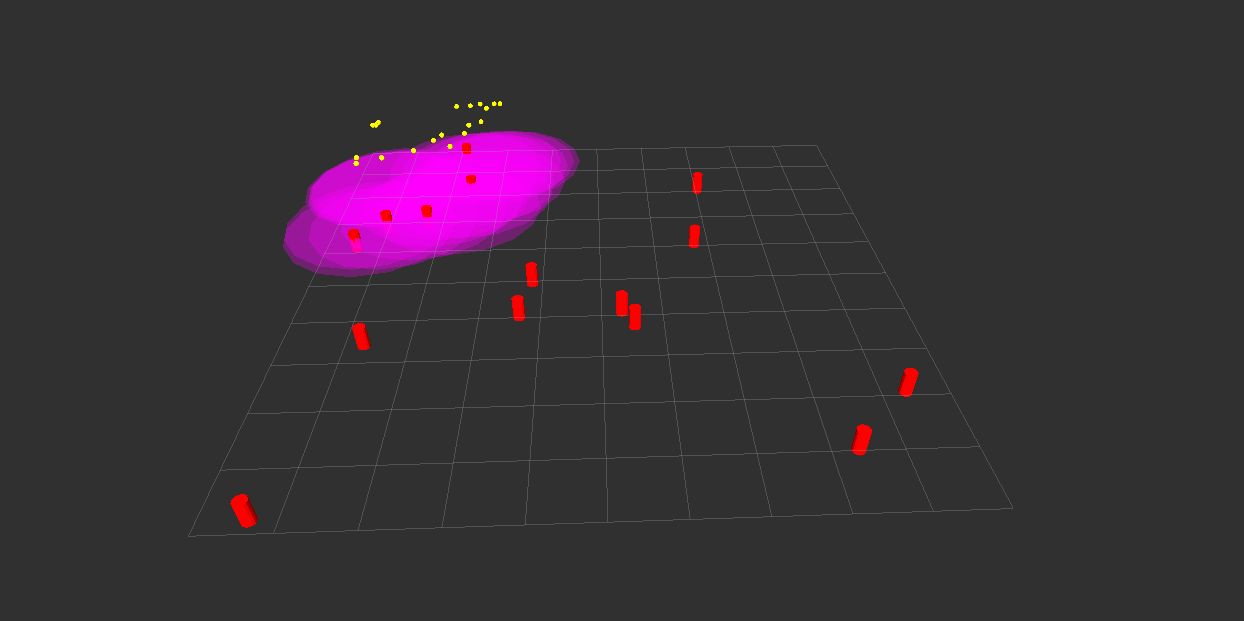
\includegraphics[width=2.5in]{figs/rover1.png} &

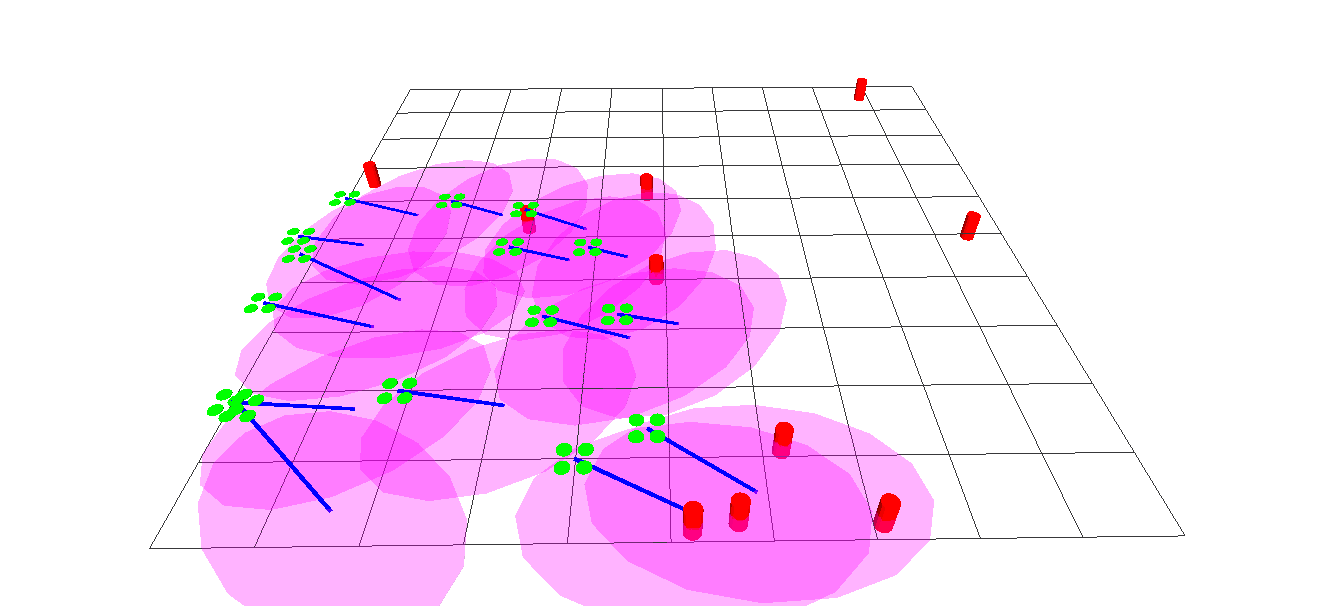
\includegraphics[width=2.5in]{figs/rover2.png} \\

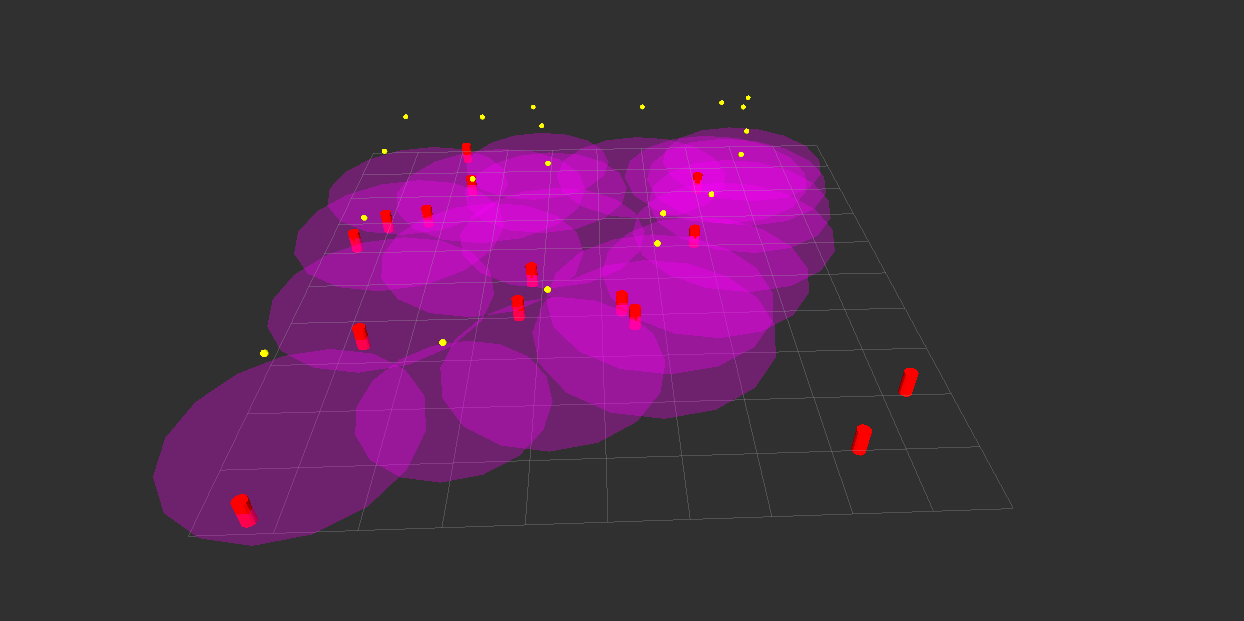
\includegraphics[width=2.5in]{figs/rover3.png} &

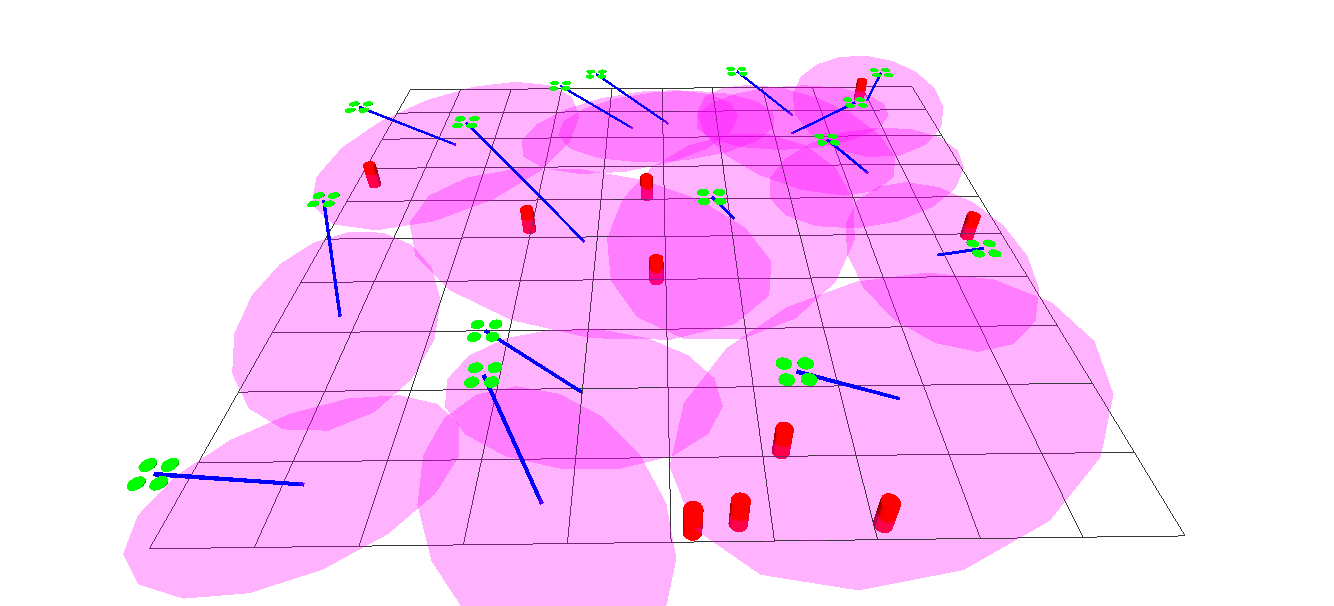
\includegraphics[width=2.5in]{figs/rover4.png}

\end{array} $$

\end{center}

\caption{The quadrotors filling up the search space}

\label{fig:cover}

\end{figure}

\subsection{Determining the altitude}

To determine the altitude, one must solve a non-linear optimization problem
that tries to optimize the height of the quad by maximizing the sensor quality
and minimizing the risk.  This is done by modelling the sensor quality and the
risk as functions parametrized by the altitude, and combining them together
into an objective function that is then maximized.

\paragraph{Sensor Quality}

To model the sensor quality, a few assumptions were made. Firstly, that there
is an optimal distance away from a tracked object such that the sensor would
have the highest quality. For example if one was tracking a person and a tank,
the optimal distance to track a person is much less than that of a tank because
the tank is larger and moves faster. It is assumed that this optimal height is
passed into the algorithm as an argument and changed for each situation. The
second assumption that is made is that the sensor quality decreases
exponentially as the distance increases. This depends on the type of sensor
that is being used and that is why this fall off can be determined the user as
well. Below is the function used to model the sensor quality. It is a normal
distribution centred at the optimal height set by the user and has a standard
deviation representative of the range of the sensor,

$$ SQ(z) = \exp{(-\frac{(\frac{z}{ cos{\phi}} -
\mu_{sq})^2}{2\sigma_{sq}^2})} $$

where $z$ is the height of the quadrotor, $\phi$ is the angle of the camera,
$\mu_{sq}$ is the optimal height for the sensor, and $\sigma_{sq}$ is a
variable indicative of the range of the sensor.

\paragraph{Risk} 

The risk is modelled in two parts. Firstly there is an initial risk, $R_0$,
which when given an $x$ and $y$ position, returns the risk as a value from 0 to
1 inclusively. This initial risk is basically the risk of the quadrotor being
detected at the ground level. This initial risk is used to scale the risk
function as altitude increases. For instance, if a quadrotor is over a very
hostile environment, there will be a very high initial risk. This would cause
the risk as height increases to decay more slowly because the quadrotor would
need to obtain a higher altitude to have less risk. However, if there is a low
initial risk, the risk as altitude increases will decay rapidly allowing the
quadrotor to fly closer to the ground. The initial risks are determined by a
set of risk points on a 2-D grid. These risk points are known \emph{a priori}.
These points are coupled with a constant between 0 to 1 which indicates how
hostile this risk point is and a constant which indicates the range of this
threat. These points are then represented as the centres of 3-D normal
distributions which are then combined to determine the initial risk in a 2-D
plane. The equation,

$$ R_0(x, y) = \Max{r_p \in \Var{RiskPoints}} r_p.\Var{hostility} \cdot
\exp{(-\frac{\sqrt{(r_p.\Var{x} - x)^2 + (r_p.\Var{y} - y)^2}}{
2 \cdot r_p.\Var{range}^2})}$$

where $x, y$ is the location of the quadrotor, $\Var{RiskPoints}$ is the list
of risk points in the grid, $r_p.\Var{range}$ is the range of the sensor, and
$r_p.\Var{hostility}$ is a measure of the hostility of the risk point from 0 to
1 is the representation of the initial risk, or the risk at the ground level.

Given a function for the initial risk, we are able to determine the risk at an
altitude by scaling this initial risk with exponential decay as height
increases. To achieve this functional behaviour, a normal distribution has been
used with a mean of 0 and a standard deviation based on a scaling of the
initial risk. The equation,

$$ R(x, y, z) = R_0(x, y) \cdot \exp{(-\frac{z^2}{K \cdot R_0(x, y)^2})} $$

is used to model the risk in three dimensions where $x, y, z$ is the position
of the quadrotor, $K$ is a scaling constant, and $R_0(x, y)$ is the initial
risk at $x, y$.

\paragraph{Optimization}

In order to determine the height of the quadrotor, me must optimize an
objective function parametrized by the altitude that maximizes the sensor
quality and minimizes the risk. This can be modelled as,

$$ J(x, y, z) = SQ(z) - R(x, y, z) $$

and therefore to determine the optimal altitude, we must find the $z$ value
that maximizes $J$ for a given $x, y$. This is shown in the equation,

$$ \Function{DetermineHeight}(x, y) = \argmax{z \in [z_{min}, z_{max}]} J(x, y,
z) $$

where $\Function{DetermineHeight}$ takes the current $x, y$ position as
parameters and returns the $z$ value that minimizes the risk whilst maximizing
the sensor quality.  This can be solved with many open source non-linear
optimizers.  The package being used in this implementation is SciPy.  Once the
altitude needed for the quad has been determined, the new height is set and the
time grid is updated.  Since the time grid is updated and it is shared within
the swarm, the change in altitude (and therefore a change in the sensor radii)
will have reactive side effects by the swarm.  If a quad, $q$, increases it's
height, the swarm will move away from it, and if $q$ decreases it's height,
there will be more unfilled space around it and the swarm will move to fill the
new space.  These properties are what allow us to break the planning into two
parts, one algorithm determining the new $x, y$ position and orientation and
another algorithm determining the new height of the quadrotor.

The complete algorithm is shown in \textbf{Algorithm} \ref{algo:planning}. In
the algorithm, $\phi$ is the camera angle, $\alpha$ is the viewing angle of the
camera, $k$ is the step size, and $A_{M}$, $A_{m}$ are the respective
semi-major and semi-minor axes.


\begin{algorithm}[ht]

\caption{Pseudocode for Rover}

\label{algo:planning}

\begin{algorithmic}[1]

\setcounter{ALC@line}{0}

\vspace*{1mm}

\STATE $\mathcal{Q} \leftarrow \Function{GetQuadrotorList()}$
\STATE $\mathcal{T} \leftarrow \Function{InitTimeGrid()}$

\WHILE{$\Function{TrackingFinished()} = \False$}

\FOR{$q \in \mathcal{Q}$}

\STATE $t_{min}, v', \beta', \phi' \leftarrow \Function{InitDynamicVars()}$
\STATE $S_{\phi} \leftarrow \Function{GetRandomSamples}(\phi_{min}, \phi_{max})$
\STATE $S_{\beta} \leftarrow \Function{GetRandomSamples}(\beta_{min}, \beta_{max})$

\FOR{$\phi \in S_{\phi}$}

\FOR{$\beta \in S_{\beta}$} 

\STATE $(v, \bar{t}) \leftarrow \Function{GetDirection}(q, \beta, \phi, \mathcal{T})$

\IF{$\bar{t} < t_{min}$}

\STATE $t_{min} \leftarrow \bar{t}$
\STATE $\beta' \leftarrow \beta$
\STATE $\phi' \leftarrow \phi$
\STATE $v' \leftarrow v$

\ENDIF

\ENDFOR

\ENDFOR

\STATE $\begin{bmatrix}
    x' \\[0.2em]
    y' 
\end{bmatrix} \leftarrow \begin{bmatrix}
    q.\Var{x} \\[0.2em]
    q.\Var{y}
\end{bmatrix} + k \cdot \mathlarger{\frac{v'}{||v'||}}$
\STATE $z' \leftarrow \Function{DetermineHeight}(x', y')$
\STATE $q.\Var{SetPosition}(x', y', z', \beta', \phi')$
\STATE $\mathcal{T}.\Var{Update}(q)$

\ENDFOR

\ENDWHILE

\end{algorithmic}
\end{algorithm}


\section{Results}

\subsection{Experimental Setup}

The experiments seeked to show that the proposed algorithm minimizes the risk,
maximizes the sensor quality, and provides sensor coverage to a designated
area. The statistics recorded were comprised of the average percent of the
total area coverage, the average sensor quality, and the average risk. The
sensor quality and risk metrics were determined using the same functions as in
the optimization process. The percent of the total area coverage was determined
using a Monte Carlo process where a large number of random points (1000) with
$x$ and $y$ values within the search area were checked to be within any of the
sensing ellipse at each iteration. The ratio of the number of points sampled
which are within any of the sensing ellipse to the total number of points
sampled is what determines the percent total area coverage metric. For the
experiments, two different independent variables were used; the number of risk
points and the number of quadrotors. The risk points were randomly placed into
the search space however, the random generator was seeded so the experiments
would be deterministic and repeatable. Also, all of the risk points used were
assigned an associated hostility and sensor range of 1 and the width of the
search space divided by two respectively. The quadrotors all started in a
square formation at the top left of the search space. Experiments were carried
out by varying the number of risk points and the number of quadrotors such that
each number or quadrotors run on every configuration of risk points. The number
of risk points varied from 1 to 21 with a step of 2 and the number of quads
varied from 1 to 26 with a step of 5. Each configuration was run for 1000
iterations and each configuration only needed to be tested once because the
process is deterministic. 

\end{document}
